
\section{Effectiveness as a platform \& navigations-per-add}

\subsection{Definitions}

A \textbf{navigation} is defined as

\onehalfspacing
\begin{itemize}
  \item a search, or
  \item a click on an instructor’s name, or
  \item a click on a crosslisted or prerequisite course link
\end{itemize}
\doublespacing

\noindent The \textbf{navigations-per-add} metric is the number of navigations taken by a user (within one session) before a section was added. 

To illustrate this metric, imagine that a user searches for ``{\tt csc}'' (one navigation so far) and begins to scroll through the list of courses. The user sees that Philip Guo is teaching CSC 210 and clicks on his name (two navigations so far), and then adds the section for CSC 210. \emph{A navigations-per-add of 2 is tallied for that user}. The user then clicks on the prerequisite for that class, CSC 172 (one navigation so far), and adds it. \emph{A navigations-per-add of 1 is tallied for that user}. The user then opens the list of labs embedded in 172 and adds one of them. \emph{A navigations-per-add of 0 is tallied for that user.} (Note that a value of 0 can also occur when a user scrolls through a list of courses and adds more than one of them without leaving the page.)

\subsection{Trends}

\begin{figure}
  \centering
  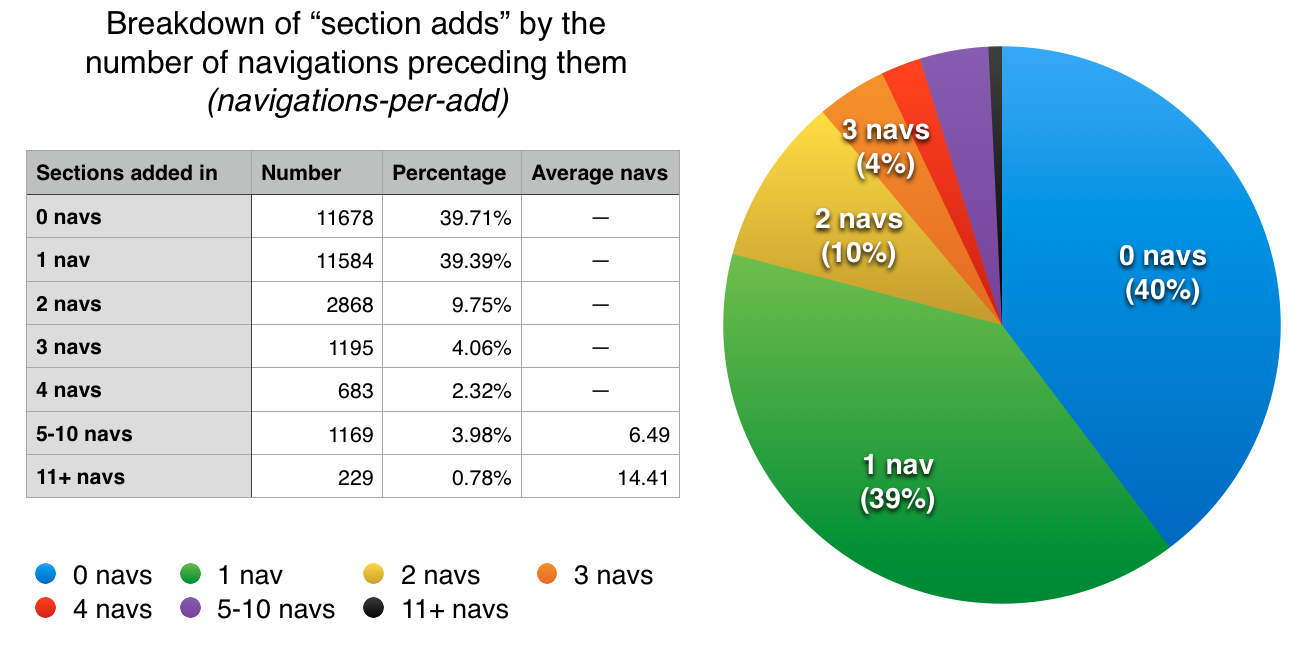
\includegraphics[width=1.0\textwidth]{images/graph/combined_navs}

  \caption{Frequency of different navigations-per-add values}
  \label{fig:navs-combined}
\end{figure}

Figure \ref{fig:navs-combined} takes the navigations-per-add for every time a course was ever added by any Skedge user.


\subsection{Breaking them apart}

  behavioral patterns
  Direct search for specific course
  Discovery, browsing, exploring

  \subsubsection{Direct searches}

  \begin{figure}
    \centering
    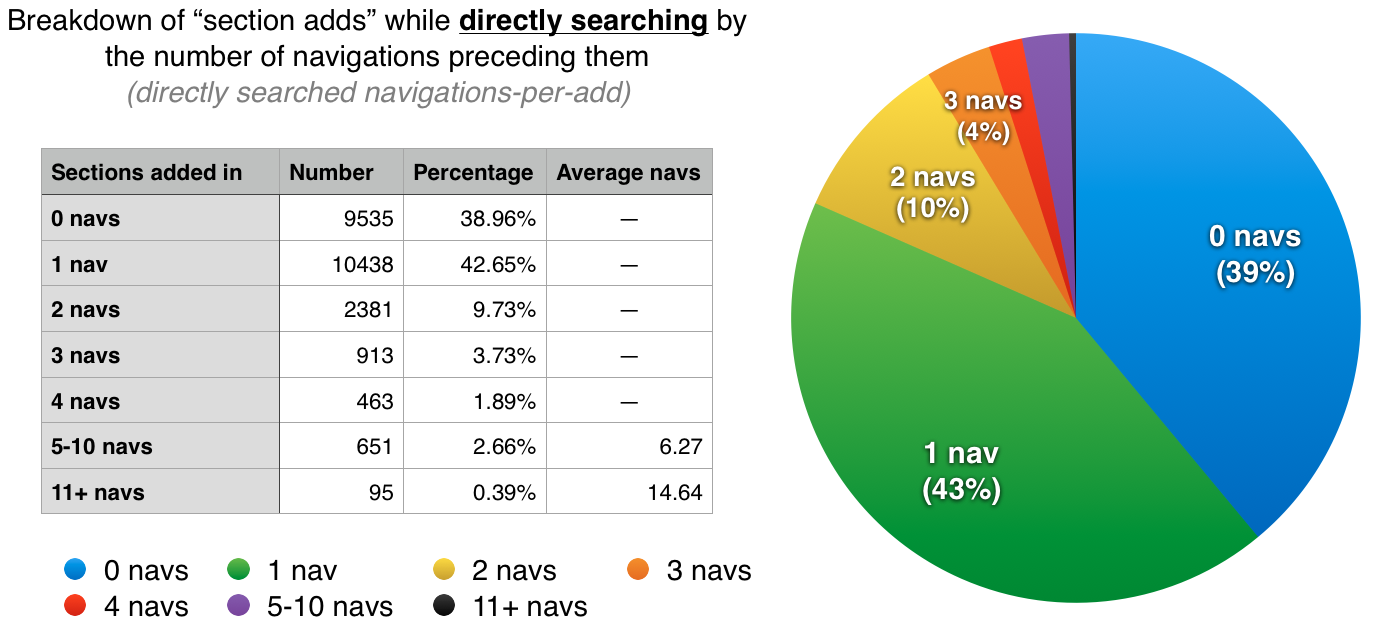
\includegraphics[width=1.0\textwidth]{images/graph/direct_navs}

    \caption{Etc}
    \label{fig:searchtypes}
  \end{figure}

  Why would 0-navs be so common with direct searches? 64\% of them subsections!

  \subsubsection{Browse}

  \begin{figure}
    \centering
    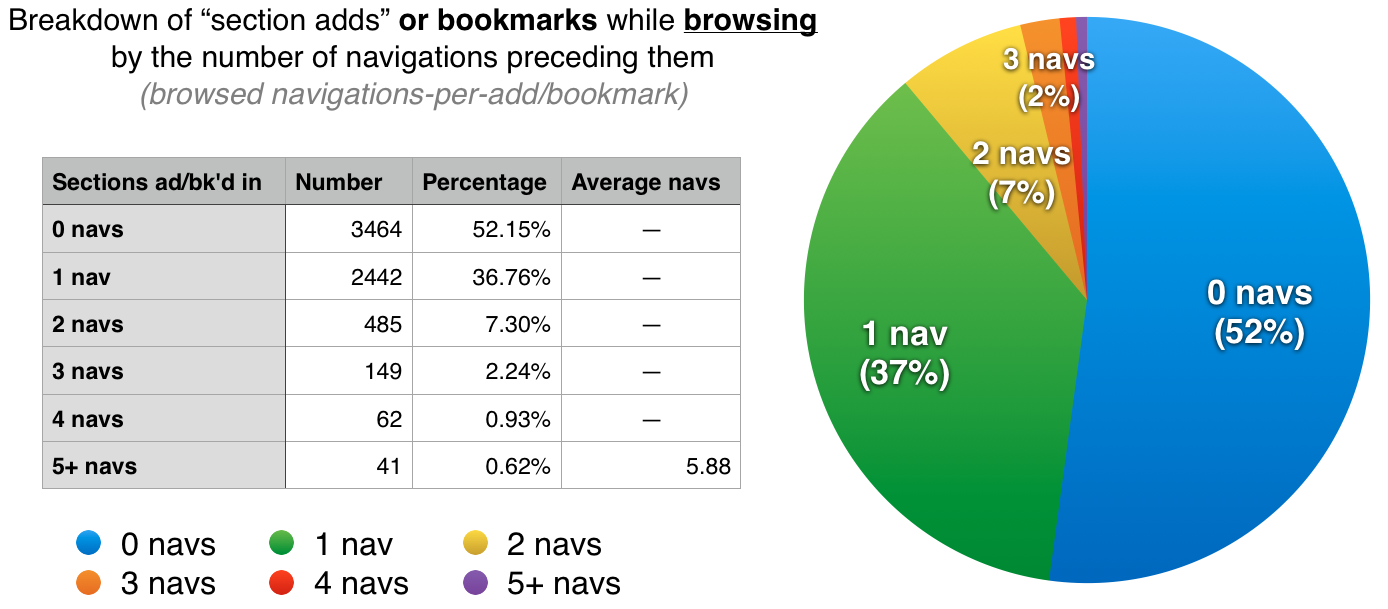
\includegraphics[width=1.0\textwidth]{images/graph/browsed_navs}

    \caption{Etc}
    \label{fig:searchtypes}
  \end{figure}

  As expected, the 0-navs were mostly maincourses (62\%)
